\documentclass{mathbook}
\usepackage{setspace}
\usepackage{graphicx}
\usepackage{hyperref}
\usepackage{amsmath}
\usepackage[letterpaper, margin={0.75in}]{geometry}
\title{First Submission}
\author{Edouard Des Parois Perrault}
\date{\today}
\teacher{Mada Hoteit}
\assignment{Math Book First Submission}
\subtitle{A Symphony of Math}
\course{Grade 11 Enriched Mathematics IB A\&A Year 1}
\school{Lower Canada College}
\schoolLogo{images/LowerCanadaCollege.jpg}
\seal{images/edouard-seal-v1-01.png}

\pagestyle{fancy}
\fancyhead{}
\makeatletter
\fancyhead[LE,RO]{\@author}
\fancyhead[RE,LO]{\textbf{\@title}}
\makeatother

\begin{document}
    \maketitle
    \onehalfspacing
    \section{Summary}
    Du Sautoy begins his narrative by introducing us to a mathematician named David Hilbert. He draws our attention to a particular presentation Hilbert gave in August 1900; during the International Congress of Mathematicians in Paris that year, Hilbert challenged his audience with a set of unsolved problems he believed should direct mathematical research for the century to come. Although there was no official time limit and no material prize, the game was on, and all hoped solutions to the 23 problems would surface prior to the end of the century. \cite{2011} In spite of the efforts of countless mathematicians, however, several of these problems remain unsolved today. \par
    
    Though that's not to say that the excitement surrounding them has died down. Quite the contrary in fact, it has only increased over the years, partly thanks to the Clay Mathematical Institute's efforts. In the year 2000, the Institute defined a smaller list, made up of the leftovers of Hilbert's list, known as the millennium problems. These problems provided mathematicians with an incentive even greater than the fame attached to Hilbert's: it promised fortune too. A monetary prize of one million dollars was, and still is, promised to anyone who solves just one of these problems. \cite[p.~15]{Sautoy2003} Du Sautoy's books is centered around one of these problems, known as number eight on Herbert's original list, number two on Clay's list, or simply as the `Riemann hypothesis'. \cite[p.~1]{Sautoy2003} This problem is a recurring motif throughout Du Sautoy's narrative, and is the glue that holds this incredibly intricate story together. It is the instrument through which Du Sautoy plays us the music of the primes.\par 

    In many respects, \emph{The Music of the Primes} is like a police novel; the detective looks for clues and evidence in order to help him identify suspects, but remains unsuccessful at uncovering the true identity of the murderer until the very end. It's the suspense and the excitement of not knowing for sure who the culprit is that makes the narrative interesting. What fun would it be if the identity of the murderer was revealed at the very beginning? Answers to mathematical problems can be just as cunning as the serial killers that take on the role of villains in many of such books, for after a problem has been identified, its solutions avoid detection much like an expert thief; they hide in the shadows and travel only at night, such that their interception is nearly impossible. That said, in spite of these rather striking similarities, Du Sautoy's narrative differs from classic murder stories in one fundamental aspect, notwithstanding the absence of murder and death in a mathematical proof, of course; in the case of a murder mystery, the justification for solving the case is rather clear; crime is a social ill and must be prevented. Conversely, in the context of a mathematical mystery such as the Riemann Hypothesis, the justification for its pursuit isn't so lucid. Why don't I just read \emph{Murder on the Orient Express} \cite{Christie1934} if I want a good murder story?
    
    Admittedly, although there are similarities between the two genres, \emph{The Music of the Primes} is not the ideal read for someone solely interested in murder and mystery. Fortunately however, readers don't need to have a PhD in math to understand the story either, for Du Sautoy  recognizes that the Riemann Hypothesis is not understood immediately by the common mortal. In fact, it is this ability of his to explain the problem in such a methodic and clear manner that makes \emph{The Music of the Primes} such an interesting read. At first, I feared that he may confine his justification to ``the Riemann Hypothesis seeks to understand the most fundamental objects in mathematics –– prime numbers'' \cite[p.~5]{Sautoy2003} Although this does answer the original question, it simply shifts the blame to another; why are \emph{primes} of any importance in the first place? Du Sautoy, however, has no intention to stop there, and consecrates several additional pages to responding to this second question. The answer, according to the author, is twofold. First, some study primes simply by virtue of their beauty and their mystery; prime numbers have both fascinated and frustrated mathematicians due to their inability to understand their underlying patterns. As Du Sautoy himself puts it, ``Randomness and chaos are anathema to the mathematician'' \cite[p.~7]{Sautoy2003} This passion for the aesthetic, however, is not something that is shared by all. Austria, for instance, found prime numbers so useless that it converted tables of prime numbers into cartridges for its use in its war against Turkey. \cite[p.~47]{Sautoy2003} Fortunately, for those who fail to see beauty in numbers, Du Sautoy also brings up another use of primes; providing security in the world of commerce and security. \cite[p.~11]{Sautoy2003} With these two motives in mind––to understand primes for both their beauty and utility––Du Sautoy ushers us into a vessel that subsequently takes us on a journey through the history of prime numbers, the mathematicians that worked on them, and the mathematical landscape that they came out of their research. Du Sautoy's vessel blasts off into the mathematical sky with its final destination clearly labelled on the map laid on its bridge:~the Riemann Hypothesis.
    
    Our first destination is Germany, where we encounter Gauß. There is a plethora of interesting characters that are mentioned throughout this book, but Gauß is by far one of the most fascinating members of the mathematical society, even today. Gauß gained considerable popularity when, in 1801, he published a series of calculations that predicted the position of the planetoid Ceres. \cite[p.~19]{Sautoy2003} Ceres had been recently discovered earlier that year by an astronomer named Giuseppe Piazzi, but its orbit had caused it to vanish shortly thereafter. This was a common occurrence with celestial objects, but it meant that mathematicians and astronomers had to subsequently engage themselves in a strange game of hide and seek; they needed to predict when and where it would appear next. In the end, Gauß emerged victorious, as his prediction ultimately proved to be the closest to the truth. \cite{Weiss1999} 

    Our next destination is not a country, but a topic; Du Sautoy proceeds to take us through an exploration of proof. He explains how the idea of mathematical proof, a concept that we take for granted today, has evolved over the course of the years. Du Sautoy begins by introducing us to a man by the name of Pierre de Fermat. Today, Fermat is known as a talented mathematician, but back in his day, he was simply known as a judge. Math, to Fermat, was not an occupation, but a hobby. To him, proof wasn't so important; if a theorem was true so far as Fermat could count, it was always true. Several centuries prior to Fermat's time, however, mathematicians had a very different approach to solving problems. In the textbook \emph{The Elements} by Euclid, for instance, there is a very well-known proof that there are infinitely many primes. This proof uses a method called \emph{reductio ad absurdum}, a form of proof by contradiction. \par
    
    Just as the idea of a proof has been subject to many amendments throughout the history of math, so has the very essence of the proofs themselves. Prior to the invention of algebra, mathematicians often relied on geometric proofs instead, such as the proof for the sum of an infinite infinite geometric series such as \(\frac{1}{2} + \frac{1}{4} + \frac{1}{8} + \cdots = 1\) shown in Figure \ref{fig:infinite-geometric-series}. \par
    
    Today, in an age of space travel, computers, and quantum theory, numbers outside of our computational reach seem closer than ever, and knowing their properties without needing to calculate them becomes a great asset. Algebraic, and not geometric, proofs have become the necessary rite of passage of a proof from conjecture to theorem.\par

    \begin{figure}
        \centering
        \caption{Sum of an Infinite Geometric Series \cite{Matteo}}
        \label{fig:infinite-geometric-series}
        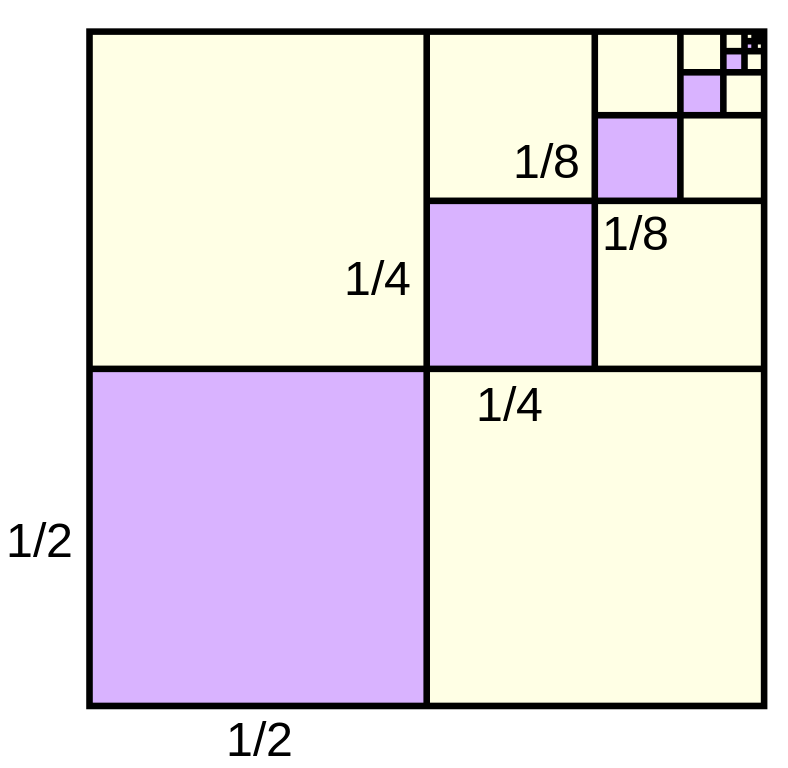
\includegraphics[scale=0.1]{images/infinite-geometric-series.png}
    \end{figure}

    Next, Du Sautoy's voyage takes us to pre-revolutionary Europe. Then, monarchs such as Peter the Great and Catherine the Great \cite{OldenbourgIdalie2020} had begun to appreciate mathematics, the sciences, and the arts. This was a complete 180 degree revolution, considering that such governments had been oppressing science for centuries. These monarchs funded the research of mathematicians such as Leonhard Euler. \cite[pp.~41-42]{Sautoy2003} Euler was also attracted by the strange light of prime numbers, and attempted to find a formula capable of producing them. Unfortunately, even he proved unsuccessful in that regard, and concluded that prime numbers were one of ``the mysteries that the human mind will never penetrate.'' \cite[p.~42]{Sautoy2003} \par
    
    Euler and Gauß's existence may have overlapped for only a short time, but they were united in their obsession with primes. Gauß too attempted this problem with a unique approach. Instead of trying to calculate the numbers themselves, he sought to find a formula capable of solving their density. When Gauß was very young, he found that there was a connection between prime numbers and logarithms, and created a formula to determine the amount of primes up to \(n\): \(n\log n\). This formula was not equal to the exact density of primes, but was a reasonable guess, and was unique in that Gauß was the first to approach the search for primes in this way. Gauß never published this discovery, however, and when the mathematician Adrien-Marie Legendre published a similar formula and claimed he had been the first to make this discovery, a conflict erupted between him and Gauß. Mathematicians tend to have strange ideas for competitions, and this gave them great inspiration. The game was on; who could create a formula capable of predicting the amount of primes up to \(n\) the most accurately? Although this particular challenge was not associated with a one million dollar prize like the millennium problems, the mere tension between the two mathematicians was enough to launch them in a marvelous race. In the end, Gauß's revised formula, the logarithmic integral \(Li(n)\), proved to be the closest to the true amount of primes up to \(n\), especially with large values of \(n\). \par
    
    Now, Du Sautoy's vessel takes a temporary break from Gauß in order to shed light on the story of a mathematician named Bernard Riemann. Riemann's story, as far as Du Sautoy is concerned, begins in the University of Berlin, where Riemann was first exposed to math. After having passed his final examinations, he sought to pursue his studies in the field, but much to his chagrin, was directed by his father to the small and quiet University of Göttingen instead in order to become a clergyman. \cite[p.~65]{Sautoy2003} Once there, however, Riemann was drawn towards mathematics and physics in lieu of theology, and eventually dedicated himself completely to math with the blessing of his father. After several years in the small town, Riemann returned to Berlin, where he was influenced by an idea that was gaining increasing traction amongst the mathematicians of the time: imaginary numbers. \par

    When writing about mathematicians that lived between 1777 and 1855, it seems impossible not to mention Gauß, for he seems to have had an impact on almost every mathematician of his time. Imaginary numbers are the solution to the equation \(x^2 = -1\), and had first been described in detail by none other than Gauß himself in his doctoral thesis of 1799. \cite[p.~69]{Sautoy2003} Other mathematicians such as Augustin-Louis Cauchy also quickly discovered that these strange numbers produced interesting results when inputted into various functions, such as sine waves, for instance. Today, sine waves with an imaginary part are called complex sinusoids, and have major applications in communication and signals. \cite{Veen2014} Filled with new ideas about imaginary numbers, Riemann returned to Göttingen in order to study under Gauß after having spent some time in France. \cite[p.~74]{Sautoy2003} Shortly after Riemann obtained his doctorate, Gauß passed away. It is with the death of Gauß, however, that the real story begins, for it is shortly thereafter that Riemann began his work on what would become the crux of the Riemann Hypothesis: the zeta function.

    \section{Reflection}

    \subsection{On RSA and Cryptography}

    ``\dots without the power of prime numbers there is no way \dots business could exist,'' according to Du Sautoy, \cite[p.~11]{Sautoy2003} and this is very true. Although at first glance, math may be rather benign, its usage in cybersecurity has given it a role at the forefront of both digital privacy, business, and crime, for the better and for the worse. This is thanks to prime numbers. As someone with an interest in computer science who has experimented with different implementations of cryptographic systems. I felt obliged to touch upon this subject in my reflection.\par
    
    The only way to determine for sure whether a number is prime is to divide it by all integers up to its square root. This is simple enough for a number such as 5 or 11, but gets rather complicated for larger numbers. Hence, if information is converted into a number and somehow multiplied by primes, it becomes impossible to find this original number unless the prime factors are known. In fact, it is based upon this idea that an algorithm, which is now referred to as RSA, was developed. RSA is heavily employed in cryptography, a discipline that solely concerns itself with securing information, whether this be computers or bank accounts. Communication over the web, for instance, is done through channels secured with RSA. RSA is essentially what is called a \emph{one-way} function. \cite{Lake2018} The security of RSA stems from the fact that it takes an astronomically large amount of computational power to reverse a one-way function and to determine the original prime factors. All in all, although historically, primes have been studied simply because of their aesthetics, it is their complexity that makes them effective tools to outsmart devices capable of performing thousands of mathematical operations per second, such as a computer. As Du Sautoy himself puts it, ``The security of RSA depends on our ability to answer basic questions about prime numbers'' \cite[p.~12]{Sautoy2003}

    \subsection{A Refutation of Objective Mathematics}

    Is mathematics an objective reality? Is there something that exists at a more fundamental level than math? If there were no humans to count, would numbers and quantities still exist? This is very much an open question, and Du Sautoy seems to be of the opinion that there exists some from of objective reality. Math is math, and whether humans are there are not, two and two will make four. In fact, in his book, Du Sautoy quotes the mathematicians G.~H.~Hardy and Alain Connes in writing that ``317 is a prime not because we think so, or because our minds are shaped in one way or another, but \emph{because it is so}, because mathematical beauty is built that way \dots There exists a mathematical reality outside of the human mind, a raw and immutable reality \dots at the heart of this world we find the unchaining list of primes.'' \cite[p.~7]{Sautoy2003} \par

    In many respects, answering this particular question is much like asking ``If a tree falls and no one hears it, does it make a sound?'' If there are two stones, but no one is there to count them, are there really two stones? I would argue that there is no reality outside of math, for math is defined by the human mind. Objects do not simply exist, they are brought into existence. Take the list of primes, for instance. What part of it is considered ``immutable''? The numerals themselves? Certainly not, for there are many other ways to express the values 3 or 7, such as perhaps III or VII. The definition of what it means to be a prime? I would argue that this argument falls just as easily, as whether or not a number is prime is a \emph{definition} with which we have come up as humans. Chris K. Caldwell and Yeng Xiong from the Waterloo Department of Mathematics and Statistics, for instance, state that ``whether or not a number (especially unity) is a prime is a matter of definition, so a matter of choice, context and tradition, not a matter of proof.'' \cite{Caldwell2012} We \emph{defined} a prime number as being a number greater than 1 that can only be divided by one and itself, but nothing stops us from expanding this definition. Of course, there are practical reasons for which 1 is not considered prime, but this does not prevent us from doing so. \par
    
    Further, in his book, Du Sautoy alludes to Carl Sagan's novel \emph{Contact}, where the main character receives a strange radio communication from space; a set of beeps; two beeps, followed by three beeps, followed by five beeps, and so on for the first prime numbers until 100. The scientist assumes that only an intelligent life form would be able to produce such a specific sequence, and it is thanks to this intuition that the communication is correctly identified as originating from an extraterrestrial source. That said, couldn't the aliens have  produced a sequence starting with \emph{one} beep instead of two? No one ever said the definition of what it meant to be prime was a fundamental truth, after all. Connes declares that math is a `universal language,' but how can it be so if the dictionary varies from one culture to another? \par

    Zero is also a rather special case. What does it mean for there to \emph{be} nothing? What does it mean to divide by nothing? This is a question that has confused and stumped generations of mathematicians, to the point at which some older numeral systems don't make use of zero at all. Why does $x^0=1$? Why does $0!=1$? Why does $\frac{x}{0}=\text{UNDEFINED}$? These are all matters of definition, and different cultures have a different understanding of them. Math is most definitely \emph{not} universal. That said, whether or not its existence presupposes the presence of a mind capable of processing it is another story, one that is perhaps impossible to answer, since it would force us to cease to exist. How can we think if we do not exist? After all, \(x \cdot 0 = 0\)~\dots

    \subsection{A Reflection on the Nature of Proofs}\label{proofs}

    Math and philosophy are fundamentally related through proofs. In \emph{The Music of the Primes}, Du Sautoy argues that ``proof in mathematics allows us to establish with 100 per cent certainty that facts about prime numbers will not change.'' \cite[pg.~32]{Sautoy2003} Du Sautoy says that proofs are statements so strong that they can never be disproven. The fundamental difference between math and other disciplines is that mathematical models can never become obsolete. Whereas in physics, the model of the universe has often been redesigned in order to correspond with more recent scientific discoveries, the mathematical model cannot become outdated, as its principles remain true. No matter what scientific discoveries come about, one and one will always make two. I beg to differ. \par
    
    Although it is undeniably true that math relies on something stronger than experimental evidence, that does not necessarily mean it cannot be beaten by time. As time ticks forward, errors can be found in theorems. Nothing is truly iron-clad. To this argument, Du Sautoy responds that ``Of course, there is no guarantee that there isn't a subtle error, but \dots~we generally believe that errors can be spotted in proofs without waiting many years for new evidence.'' \cite[p.~33]{Sautoy2003} At this point, I am tempted to cite Andrew Wiles's proof of Fermat's last theorem, and how it was shown that he was incorrect only \emph{after} his publication of this proof. For awhile, something false was considered to be true. In this particular situation, however, Du Sautoy's argument would still stand, since the error was found shortly after the publication of the paper; mathematical proofs are always correct since, if they have an error, this error is already written on the page, and can therefore be addressed almost immediately. \par
    
    So perhaps proofs are indeed by definition iron-clad, but there is another argument against their immortality; can we ever state with certainty that a claim based on a posteriori axioms originating from the physical world are true? The French philosopher Descartes addressed this extensively in his \emph{Meditations on First Philosophy}, \cite{Descartes1637} and believed that sensory, or empirical, information was not enough, for the existence of optic and sensory illusions suggested that it was possible for our senses to deceived us. For instance, there is no way to disprove the belief that every time we count the sides of a triangle, we are deceived into believing that there are three sides, when there are in fact two, or four, or none, or some other quantity. \cite{Newman2019} As Descartes so eloquently states, ``How do I know \dots that there is no earth, no sky, no extended thing, no shape, no size, no place, while at the same time ensuring that all these things appear to me to exist just as they do now?'' All in all, in my opinion, whether or not a mathematical proof cannot be defeated is still very much an open question, and so long as such solipsistic and perhaps even theological inquiries, such as the origin of the material world, remain unanswered, we shall never know for sure whether something like a proof is truly true.

    \newpage
    \bibliographystyle{IEEEtran}
    \bibliography{refs}
    %%% Extra %%%
    % The 19th century proved to be a unique time in Germany, for then, the new education minister sought to reform the system . \cite[p.~59]{Sautoy2003} Germany's government was not alone in this regard, however, for France's education system was also undergoing considerable change under the leadership of Napoleon Bonaparte. The main difference between the two regimes was that Napoleon encouraged professors to teach the military applications of mathematics, while those in Germany were more appreciative of the philosophical and aesthetic aspects of the subject. \cite[p.~61]{Sautoy2003} \par
    % Even as a young child, Gauß is known to have been incredibly precocious in the speed at which he grappled with complex mathematical concepts. For instance, there is a well-known story of how, when he was just 10, Gauß created a formula to find the \(n\)th triangular number, namely, \(\frac{1}{2} \cdot (N + 1) \cdot N\), impressing even his teacher.  \cite[p.~25]{Sautoy2003}
    % Du Sautoy will return to Gauß later on in his book. In the meantime, we come across a mathematician which today has been given the name Fibonacci. Fibonacci is well known due to his discovery of the Fibonacci sequence in his investigation of rabbit reproduction patterns. In addition, the Fibonacci sequence shows up in all sorts of strange places, such as the position of petals in a flower \footnote{See \cite{Numberphile2018} for a great video on this topic.} or the ratio between someone's height to the distance between their feet and their bellybutton. 
    % Today, Gauß is considered to be one of the greatest mathematical minds that existed. Although he wasn't as productive as Euler, he made several contributions to a variety of fields throughout his lifetime. These contributions include modular arithmetic, which has a role to play in RSA encryption and modern computer science. These discoveries, which he published in his book \emph{Disquisitiones Arithmeticae}, are considered to comprise the foundations for a subject we call number theory today. \cite[p.~22]{Sautoy2003}
    %  That said, Du Sautoy recognizes that the importance of primes numbers is not evident to the reader right away I personally expected Du Sautoy to provide a deeply philosophical justification, along the lines of ``because math is beautiful'' or ``because it is human nature to solve problems'' or even just ``because,'' \footnote{That's not to say that these justifications are untrue or irrelevant, for they are not, but it is undeniably true that they are rather cliche. Take Henri Pointcarte's explanation, for example; ``The scientist does not study Nature because it is useful; he studies it because it is beautiful''\cite[p.~6]{Sautoy2003}} I was pleasantly surprised to find an alternative, more pragmatic, justification. The 
    % the unknown lies within the depths of the psyche of almost every human being. Perhaps the feeling that swept the audience as Hilbert presented his problems wasn't dissimilar from the sentiment we as students experience when we are presented with a blank math competition.
    % It is therefore no surprise that Du Sautoy refrains from explaining it at the beginning of his narrative. Instead, he goes on to talk about how the world once almost thought it was solved. He narrates a joke the mathematician Enrico Bomberi made for April fools that ended up being so successful even the United States government thought the hypothesis has been cracked. He told the world that the hypothesis had been solved, even if this was far from being the case. \par
    % \footnote{It seems to be the habit of mathematicians to produce overly cryptic justifications for their intentions. Take the polymath Pierre-Simon Laplace's praise of Euler, for instance. He says ``Read Euler, read Euler, he is the master of us all.'' Although we can guess that what he means to say is that he loves reading Euler, it's almost as though it takes a proof in itself to determine for sure what he is saying!}
\end{document}